%!TEX root = ../farid_msc_thesis.tex

\chapter{Results}
\label{ch:results}

\subsection{Models Prediction of Categories}
\subsubsection{Multinomial Naive Bayes Classifier}
Some scores obtained:
\texttt{.\\
             precision    recall  f1-score   support \\
\\
       -1.0       0.69      0.49      0.57       859\\
        1.0       0.62      0.79      0.69       904\\
\\
avg / total       0.65      0.64      0.63      1763\\
}

\begin{figure}[h]
	\label{fig:nbConfusion}
	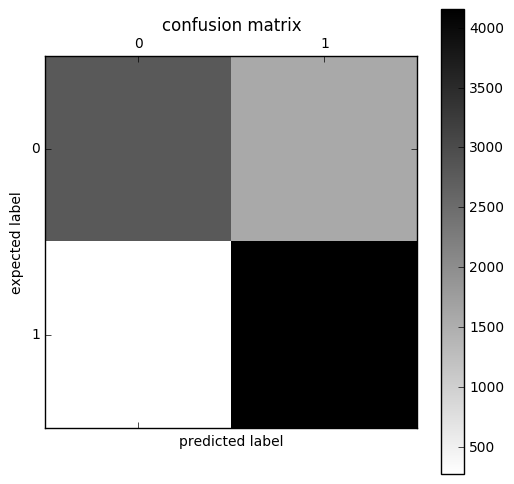
\includegraphics[width=\textwidth]{badConfusionMatrixNB.png}
    \caption{Confusion Matrix for Multinomial Naive Bayes Classifier.}
\end{figure}

Next, we plot the precision vs training samples:

\begin{figure}[h]
	\label{fig:correlaciones}
	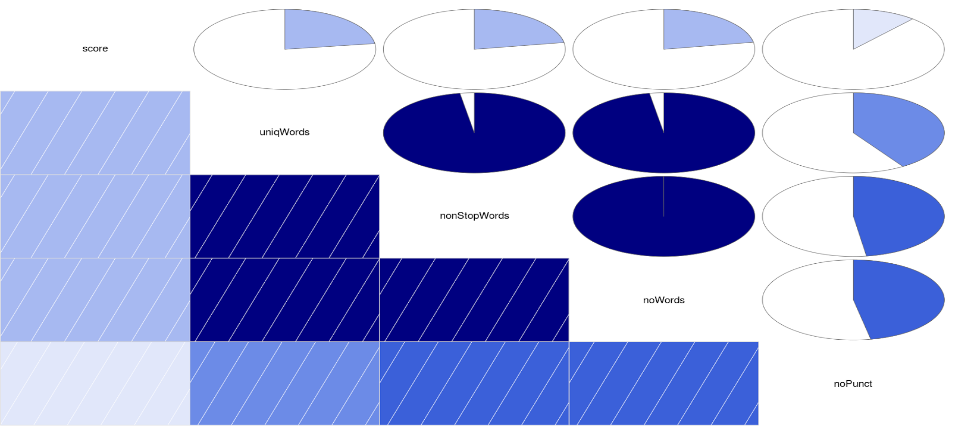
\includegraphics[width=\textwidth]{correlations_image_posible.png}
    \caption{Using Multinomial Naive Bayes Classifier.}
\end{figure}


%
\section{Results}
%
\begin{figure}[h]
	\label{fig:partialResults1}
	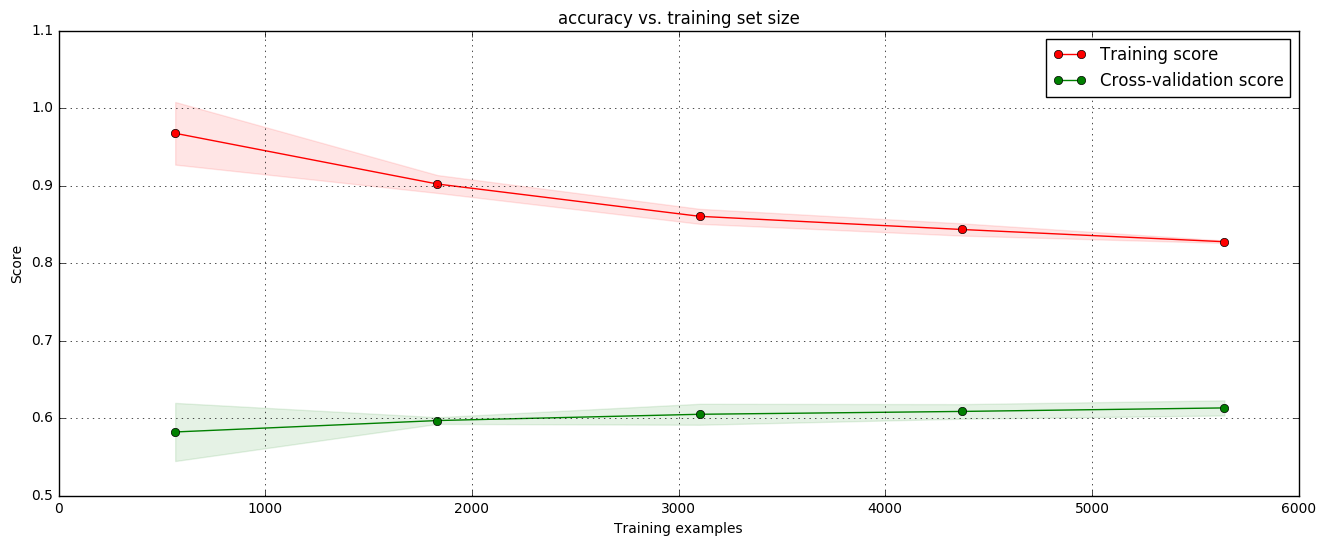
\includegraphics[width=\textwidth]{trainingAccuaracyMNaiveBayes.png}
    \caption{Accuracy Vs Training set size.}
\end{figure}


\subsubsection{Support Vector Machine}
Some scores obtained:
\texttt{.\\
     precision    recall  f1-score   support\\
\\
       -1.0       0.62      0.62      0.62       859\\
        1.0       0.64      0.64      0.64       904\\
\\
avg / total       0.63      0.63      0.63      1763\\
}